\chapter{Ingeniería de Software Ágil}

Hacer agilidad no nos asegura calidad. Para ello primero hay que asegurarse de hacer ingeniería de software además de agilidad. Hay diferentes procesos de ingeniería y podemos tomar el siguiente: descubrimiento y requerimientos (Discovery \& Requirements), análisis y diseño (Analysis \& Design), implementación y pruebas (Implementation \& Testing), integración (Integration), despliegue (Delivery) y monitoreo (Monitoring). Hay que considerar que el proceso de Ingeniería de Software, si bien es secuencial, tiene las fases que se solapan. 

\begin{figure}[h]
  \centering
  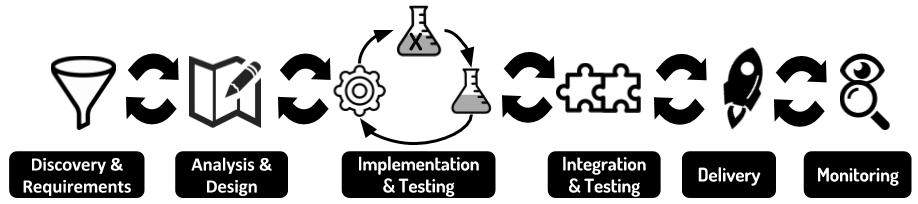
\includegraphics[width=0.99\textwidth]{PhasesOfSoftwareEngineering}
  \caption{Fases de Ingeniería de Software}
  \centering
  \label{fig:PhasesOfSoftwareEngineering} %\ref{fig:PhasesOfSoftwareEngineering}
\end{figure}

Correr este proceso bajo un marco ágil como Scrum, con prácticas ágiles es lo que podemos llamar Ingeniería de Software Ágil (Agile Software Engineering). Además es conveniente introducir la idea de prácticas continuas, es decir refinamiento continuo, testing continuo (continuous testing), integración continua (continuous integration), despliegue o entrega continua (continuous deployment \& continuous delivery) y monitoreo continuo (continuous monitoring). 
Dicho esto, tenemos que tener en cuenta cómo unir y ajustar el proceso de Ingeniería de Software con el marco de trabajo Scrum. En este sentido es que se plantea ejecutar las fases del proceso de ingeniería dentro del tren de sprints. En un equipo extremadamente autónomo y ágil, todas las fases se pueden desarrollar bajo el tren de sprints de Scrum.

\begin{figure}[h]
  \centering
  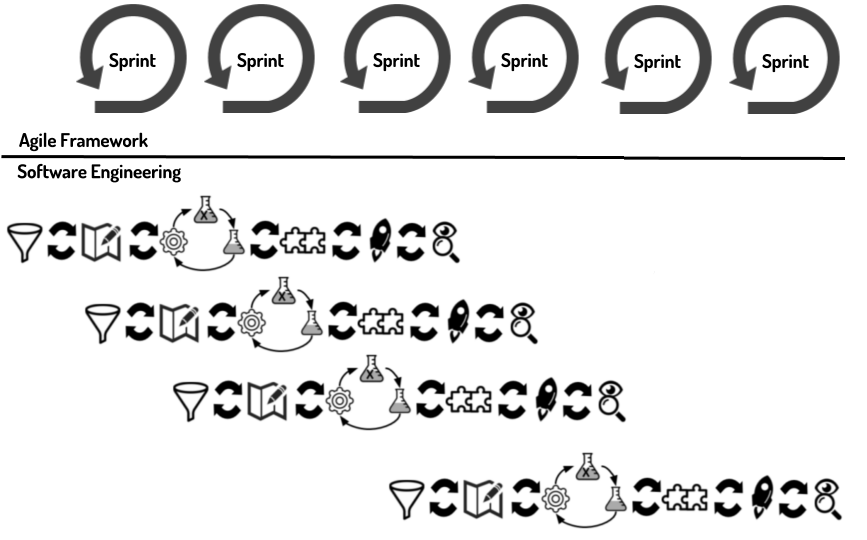
\includegraphics[width=0.99\textwidth]{AgileSoftwareEngineering}
  \caption{Ingeniería de Software Ágil}
  \centering
  \label{fig:AgileSoftwareEngineering} %\ref{fig:AgileSoftwareEngineering}
\end{figure}

